\documentclass{beamer}
\usepackage[utf8]{inputenc}
\usepackage[english]{babel}
\usepackage[T1]{fontenc}
\usepackage{lmodern}
\usepackage{amsmath}
\usepackage{stmaryrd}
\usepackage{graphicx}
\usepackage{framed}
\usepackage{listings}
\usepackage{placeins}
\usepackage{subcaption}
\usepackage{array}
\usepackage{listings}
\usepackage{hyperref}
\usepackage{xspace}
\usepackage{relsize}
\usepackage{xcolor}
\usepackage{mathpartir}

\setbeamertemplate{navigation symbols}{}

\usetheme{Berkeley}

\begin{document}

\title[Mechanistic links between cellular trade-offs, gene expression, and growth]{Mechanistic links between cellular trade-offs, gene expression, and growth}
\author{Andrea Y. Weiße et al., \emph{PNAS} vol. 112 no. 9}
\date{Théotime Grohens}

\begin{frame}
\titlepage
\end{frame}

\begin{frame}
\frametitle{Outline of the presentation}
\tableofcontents[pausesections]
\end{frame}

\section{Description of the model}

\begin{frame}
\frametitle{A coarse-grained, ODE model}
\begin{itemize}
\item Describes intracellular levels of energy, nutrients, mRNAs and proteins
\item Only 14 different variables, obeying simple differential equations obtained from chemical reactions
\item Much simpler than whole-cell models, and thus simpler to reason about
\end{itemize}
\end{frame}

\begin{frame}
\frametitle{Goal of the model}
\begin{itemize}
\item Main goal: be able to study the trade-offs that cells have to make when growing
\item Simplicity: allows us to tweak it easily and add extensions
\end{itemize}
\end{frame}

\begin{frame}
\frametitle{3 cellular trade-offs}
\begin{itemize}
\item Finite energy levels: mRNA-ribosome complexes compete for energy to translate
\item Finite ribosome levels: mRNAs compete for ribosomes to bind to
\item Finite cell mass: proteins compete for proportion of cell mass
\end{itemize}
\end{frame}

\begin{frame}
\frametitle{Description}
\centering
\includegraphics[width=0.85\textwidth]{model.png}
\end{frame}

\begin{frame}
\frametitle{Differential equations}
$$
\begin{cases}
\dot{s}_i &= \nu_{imp}(e_t, s) - \nu_{cat}(e_m, s_i) -\lambda s_i \\
\dot{a} &= n_s \nu_{cat}(e_m, s_i) - \sum\limits_{x\in \{r, e_t, e_m, q\}}n_x \nu_x(c_x, a) - \lambda a \quad (1)\\
\dot{r} &= \nu_r(c_r, a) -\lambda r + \sum (\nu_x(c_x, a)- k_b r m_x + k_u c_x) \\
\dot{e}_t &= \nu_t(c_t, a) - \lambda e_t \\
\dot{e}_m &= \nu_e(c_e, a) - \lambda e_m \\
\dot{q} &= \nu_q(c_q, a) - \lambda q \\
\dot{m}_x &= \omega_x(a) - (\lambda + d_m)m_x + \nu_x(c_x, a)- k_b r m_x + k_u c_x \quad (2)\\
\dot{c}_x &= -\lambda c_x + k_b r m_x - k_u c_x - \nu_x(c_x, a)
\end{cases}
$$
\end{frame}

\begin{frame}
\frametitle{Differential equations}
$$
\begin{cases}
\nu_{imp}(e_t, s) &= e_t\frac{v_t s}{K_t+s} \\
\nu_{cat}(e_m, s_i) &= e_m\frac{v_m s_i}{K_m+s_i} \\
\nu_x (c_x, a) &= c_x \frac{\gamma(a)}{n_x} \qquad (1)\\
\gamma(a) &= \gamma_{max}\frac{a}{K_\gamma+a} \\ 
\omega_x(a) &= w_x\frac{a}{\theta_x+a} \\
\omega_q(a) &= w_x\frac{a}{\theta_x+a}I(q) \\
I(q) &= \frac{1}{1+(\frac{q}{K_q})^{h_q}} \\
R_t &= \sum_x c_x \\
M &= \sum_x n_x x + R_t \quad (3, constant)\\
\lambda &= \gamma(a)\frac{R_t}{M}
\end{cases}
$$
\end{frame}

\section{Varying the external medium}

\begin{frame}
\tableofcontents[currentsection]
\end{frame}

\begin{frame}
\frametitle{Nutrient efficiency and chloramphenicol}
\begin{itemize}
\item Varying nutrient efficiency changes the level of available energy in the cell, impacting the 1st tradeoff
\item Chloramphenicol: antibiotic that inhibits translation, affects the 2nd tradeoff
\end{itemize}
\end{frame}

\begin{frame}
\frametitle{Experimental results}
\centering
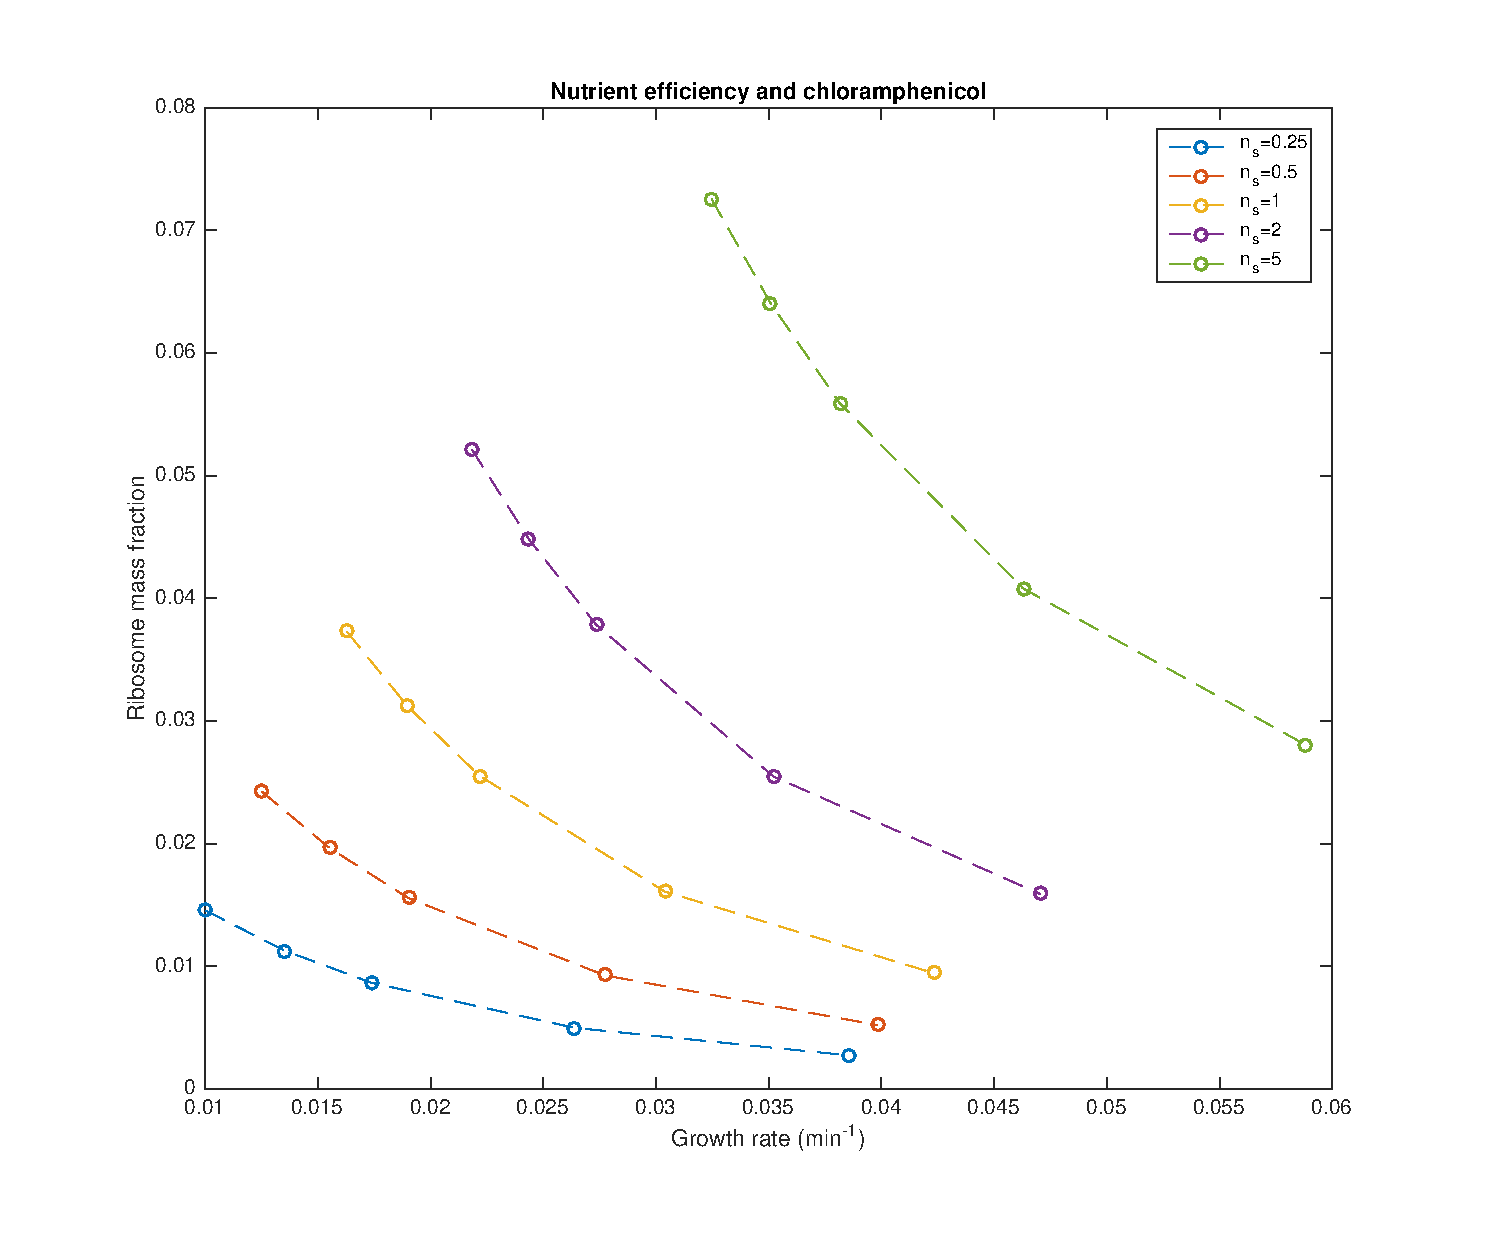
\includegraphics[width=0.9\textwidth]{chlor.eps}
\end{frame}

\section{Relative transcription rates and energy levels}

\begin{frame}
\tableofcontents[currentsection]
\end{frame}

\begin{frame}
\begin{figure}
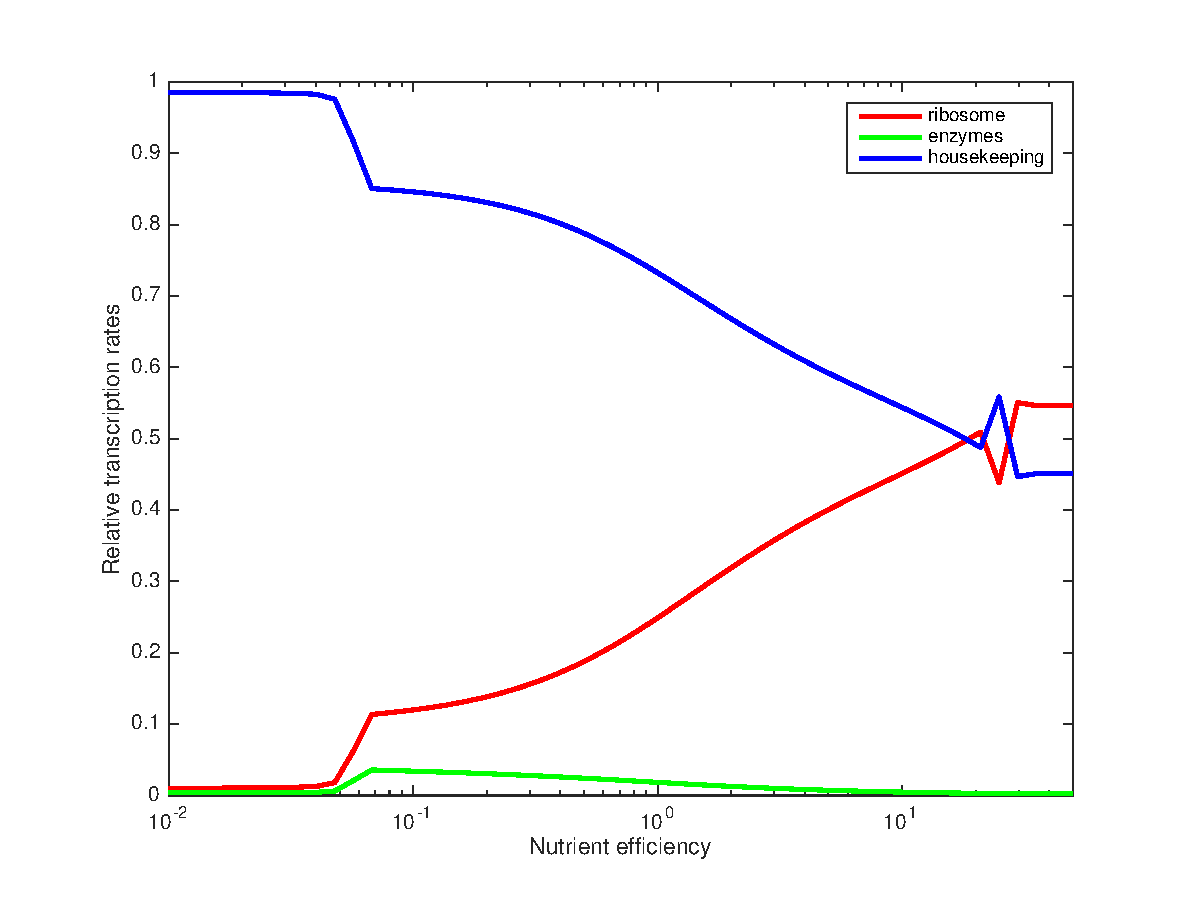
\includegraphics[width=0.9\textwidth]{transcription.eps}
\caption{Evolution of transcription rates with nutrient efficiency.}
\end{figure}
\end{frame}

\begin{frame}
\frametitle{The cell chooses what to transcribe depending on the available energy level}
\begin{itemize}
\item At low energy: make more enzymes to increase energy levels
\item At high energy: make more ribosomes to increase protein production
\end{itemize}
\end{frame}

\section{Gene dosage compensation}

\begin{frame}
\tableofcontents[currentsection]
\end{frame}

\begin{frame}
\frametitle{Gene dosage compensation}
\begin{itemize}
\item	Delete one of two paralogous genes
\item Observe the change in the expression rate
\item Responsiveness: $R(x) = \log(\frac{x^{\Delta_y}}{\delta(x,y)x^{wt}})$ 
\end{itemize}
\end{frame}

\begin{frame}
\frametitle{Experiments}
\begin{itemize}
\item Wild-type strain: with a gratuitous protein
\item Protein deletion strain: halve the protein transcription
\item Enzyme deletion strain: halve enzyme transcription
\end{itemize}
\end{frame}

\begin{frame}
\begin{figure}
\frametitle{Enzyme deletion strain}
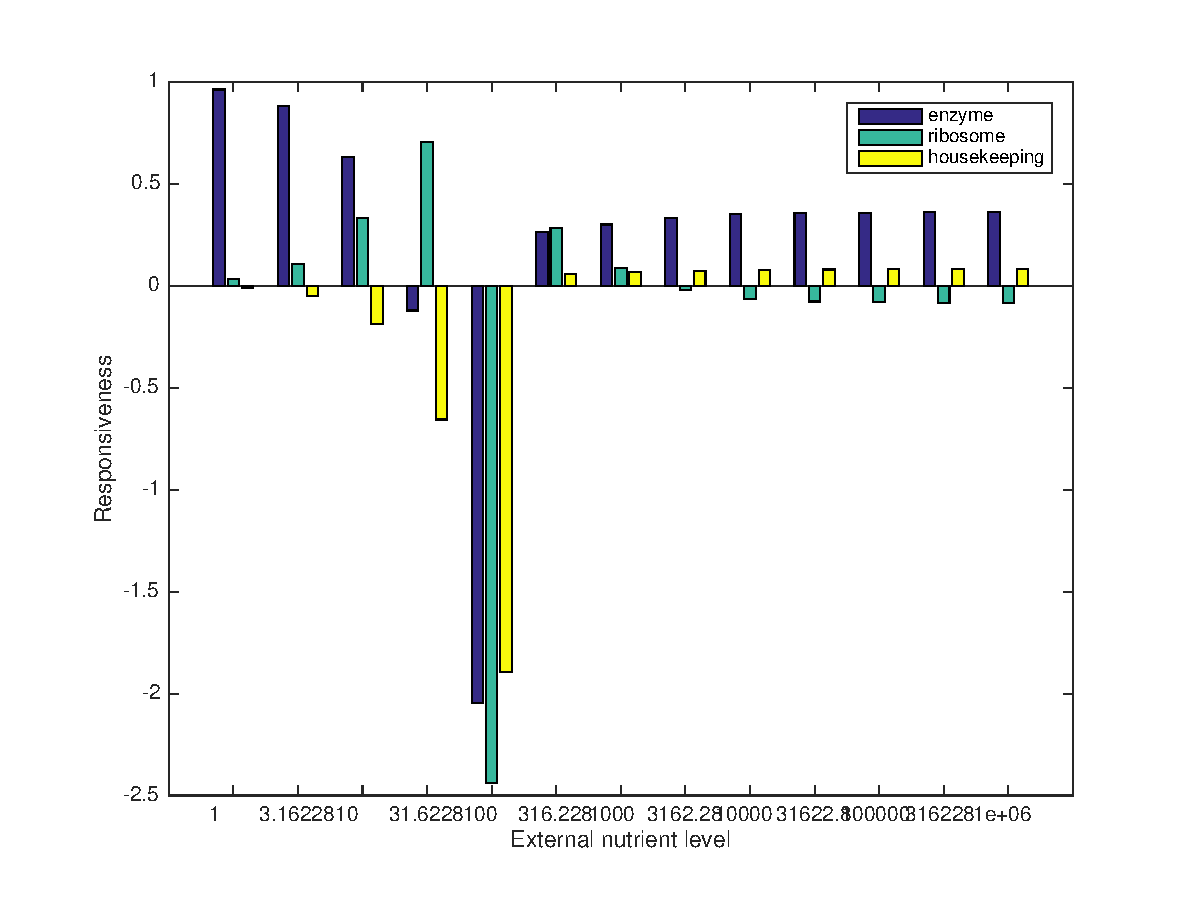
\includegraphics[width=0.9\textwidth]{enzdel.eps}
\caption{Responsiveness in the enzyme deletion strain.}
\end{figure}
\end{frame}

\begin{frame}
\begin{figure}
\frametitle{Protein deletion strain}
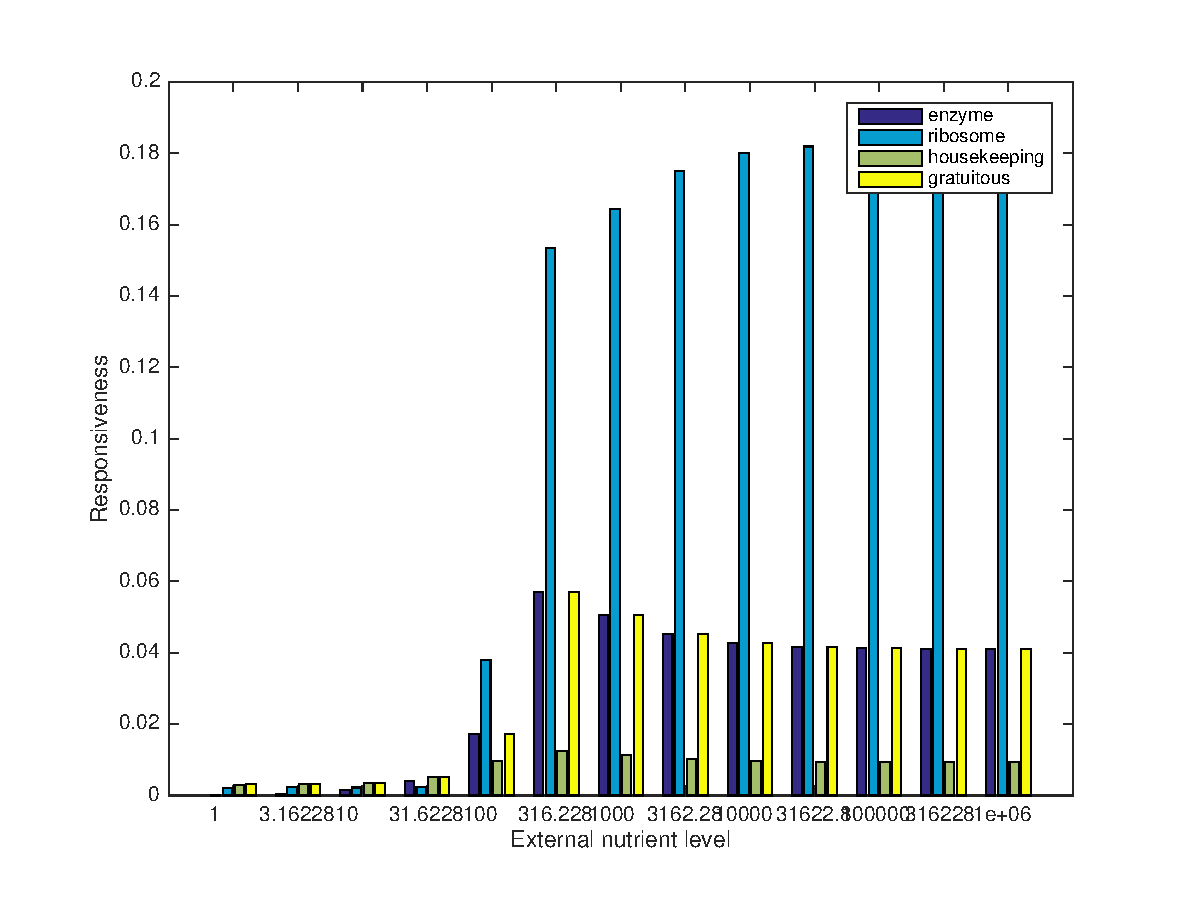
\includegraphics[width=0.9\textwidth]{gratdel.eps}
\caption{Responsiveness in the gratuitous protein deletion strain.}
\end{figure}
\end{frame}

\begin{frame}
\begin{figure}
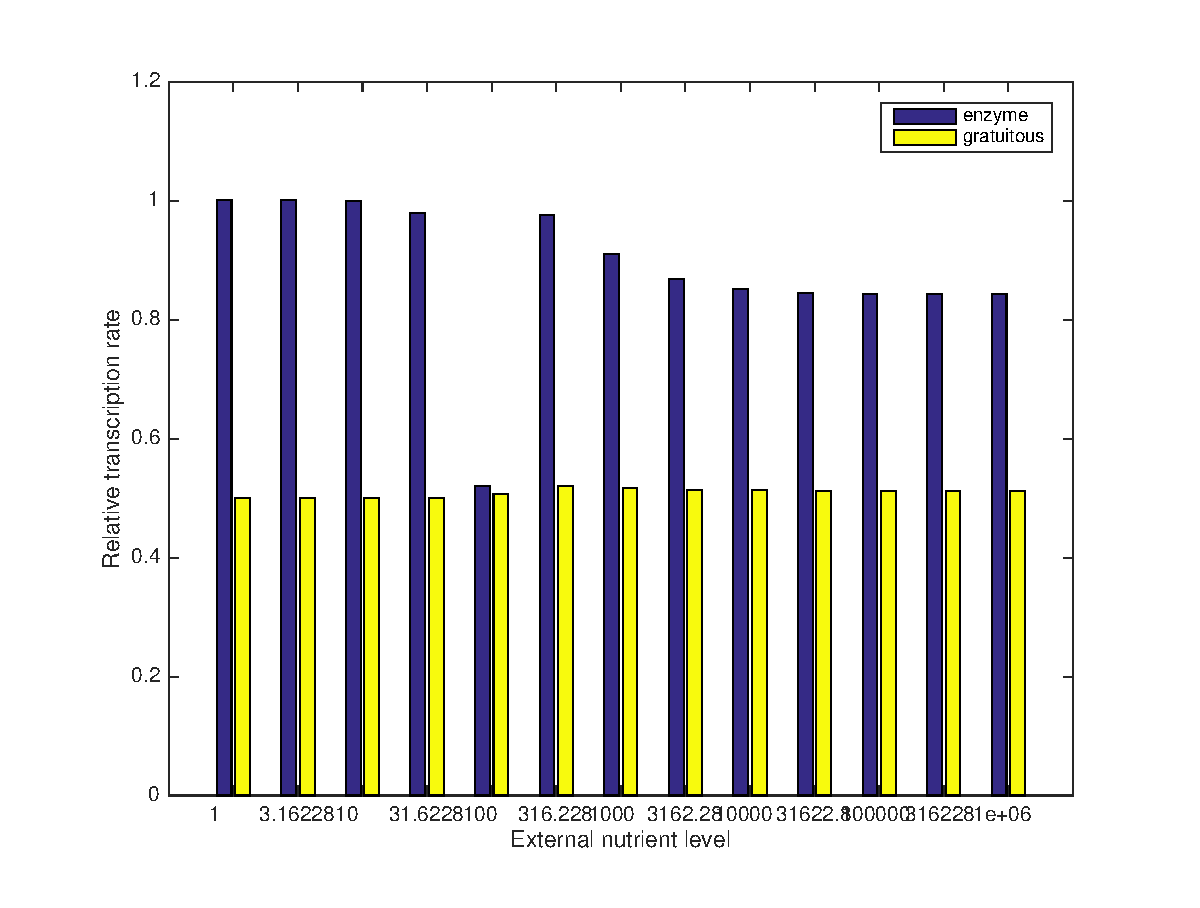
\includegraphics[width=0.9\textwidth]{reltransdel.eps}
\caption{Relative transcription rates in the deletion strains.}
\end{figure}
\end{frame}

\begin{frame}
\frametitle{Responsiveness in the paper}
\includegraphics[width=\textwidth]{resp.png}
\end{frame}

\section{Adding a synthetic circuit}

\begin{frame}
\tableofcontents[currentsection]
\end{frame}

\begin{frame}
\frametitle{The toggle switch}
\begin{itemize}
\item Two proteins: TetR and LacI
\item Inhibit each other's transcription
\item Don't interact with the metabolism apart from their use of cell resources
\end{itemize}
\end{frame}

\begin{frame}
\frametitle{Experiment}
\begin{itemize}
\item Vary the induction level of the external circuit
\item Look at the relative and absolute translation (production) of the proteins involved
\item Maximizing induction does not maximize output!
\end{itemize}
\end{frame}

\begin{frame}
\begin{figure}
\frametitle{Results}
\includegraphics[width=0.9\textwidth]{induction.eps}
\caption{Protein transcription rates and cell growth rate (in min$^{-1}$).}
\end{figure}
\end{frame}

\begin{frame}
\frametitle{Conclusion}
\begin{itemize}
\item Simple model: experiments are easier to make and to interpret
\item The effects of the trade-offs are visible even with a very simple model
\item The trade-offs interpretation does help understanding the experimental results
\end{itemize}
\end{frame}

\end{document}